\documentclass[t]{beamer}
\usepackage[utf8]{inputenc}  % to be able to type unicode text directly
\usepackage{inconsolata}     % for a nicer (e.g. non-courier) tt family font
\usepackage{amsthm,amsmath}  % fancier mathematics

\usepackage{graphicx}        % to include images
\usepackage{animate}         % to include animated images
\usepackage{hyperref,url}    % to make clickable hyperlinks
%\usepackage{minted}          % for code insets
\usepackage{array}           % to fine-tune tabular spacing
%\usepackage{bbm}             % for blackboard 1
\usepackage{soul}            % for colored strikethrough
%\usepackage{bbding}          % for Checkmark and XSolidBrush
\usepackage{mathabx}

\colorlet{darkgreen}{black!50!green}  % used for page numbers
\definecolor{term}{rgb}{.9,.9,.9}     % used for code insets


% coco's macros
\def\R{\mathbf{R}}
\def\F{\mathcal{F}}
\def\x{\mathbf{x}}
\def\y{\mathbf{y}}
\def\u{\mathbf{u}}
\def\Z{\mathbf{Z}}
\def\d{\mathtt{d}}
\def\ds{\displaystyle}
\DeclareMathOperator*{\argmin}{arg\,min}
\DeclareMathOperator*{\argmax}{arg\,max}
\newcommand{\reference}[1] {{\scriptsize \color{gray}  #1 }}
\newcommand{\referencep}[1] {{\tiny \color{gray}  #1 }}
\newcommand{\unit}[1] {{\tiny \color{gray}  #1 }}

% disable spacing around verbatim
\usepackage{etoolbox}
\makeatletter
\preto{\@verbatim}{\topsep=0pt \partopsep=0pt }
\makeatother

% disable headings, set slide numbers in green
\mode<presentation>
\setbeamercolor*{author in head/foot}{parent=none}
\setbeamercolor*{title in head/foot}{parent=none}
\setbeamercolor*{date in head/foot}{parent=none}
\defbeamertemplate*{footline}{infoline theme}
{
  \leavevmode%
  \hfill\color{darkgreen}
   \insertframenumber{} / \inserttotalframenumber\hspace*{2ex}
  \vskip0pt%
}
\mode<all>
\setbeamertemplate{navigation symbols}{}

% select red color for strikethrough
\makeatletter
\newcommand\SoulColor{%
  \let\set@color\beamerorig@set@color
  \let\reset@color\beamerorig@reset@color}
\makeatother
\newcommand<>{\St}[1]{\only#2{\SoulColor\st{#1}}}
\setstcolor{red}





\begin{document}

\begin{frame}[plain,fragile]
\begin{verbatim}









            FOCUSING 









eml
\end{verbatim}
\end{frame}

%\begin{frame}\ttfamily
%FOURIER ANALYSIS IN ONE SLIDE\\
%=============================\\
%
%\medskip
%
%Definitions:\\
%
%\medskip
%
%	\begin{tabular}{|l|l|}
%		\hline
%$\ds\widehat{f}(y)=\frac{1}{\sqrt{2\pi}}\int f(x) e^{-ixy}\d x$
%&
%$\ds\widecheck{f}(y)=\frac{1}{\sqrt{2\pi}}\int f(x) e^{ixy}\d x$
%\\
%	\tiny\color{gray} Fourier transform &
%	\tiny\color{gray} inverse Fourier transform \\
%		\hline
%%	& \\
%$\ds (f*g)(y)=\int f(x) g(y-x)\d x$
%&
%$\ds (f\star g)(y)=\int \widebar{f(x)} g(y+x)\d x$
%\\
%	\tiny\color{gray} convolution &
%	\tiny\color{gray} cross-correlation \\
%		\hline
%\end{tabular}
%
%\vfill
%
%Properties:\\
%
%\medskip
%
%	$\widecheck{\widehat{f}}=f$
%	$\qquad$
%	$f*g=g*f$
%	$\qquad$
%	$f\star g\neq g\star f$
%	$\qquad$
%	$f*(g*h)=(f*g)*h$
%	$\qquad$
%	$f\star (g\star h)\neq(f\star g)\star h$
%	$\qquad$
%	$\widehat{f*g}=\widehat{f}\widehat{g}$
%	$\qquad$
%	$\widehat{f\star g}=\widehat{f}\widebar{\widehat{g}}$
%
%\end{frame}

\begin{frame}[plain,fragile]
\begin{verbatim}
CONTENTS
========

0. Exploration of a radar image of Rotterdam
1. Principles of S.A.R. imaging
2. Focusing experiments
3. Goals and open problems
\end{verbatim}
\end{frame}



\begin{frame}\ttfamily
AN EXAMPLE RADAR IMAGE: OVERVIEW\\
================================\\
$ $\\

1 SLC datum = 6 complex images of size 20.000 x 15.000 \\
	{\color{gray} (vv, vh) x (iw1, iw2, iw3)}\\

	32 bits per complex sample $\approx$ 8GB

	\vfill

\begin{tabular}{cc}
	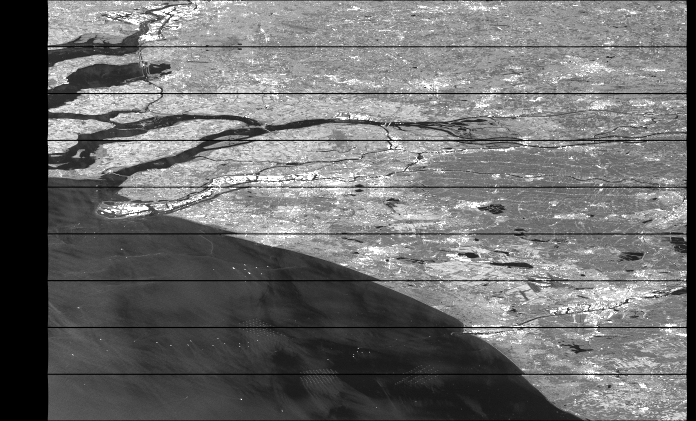
\includegraphics[width=0.5\linewidth]{f/slc_nvv_whole.png}
	&
	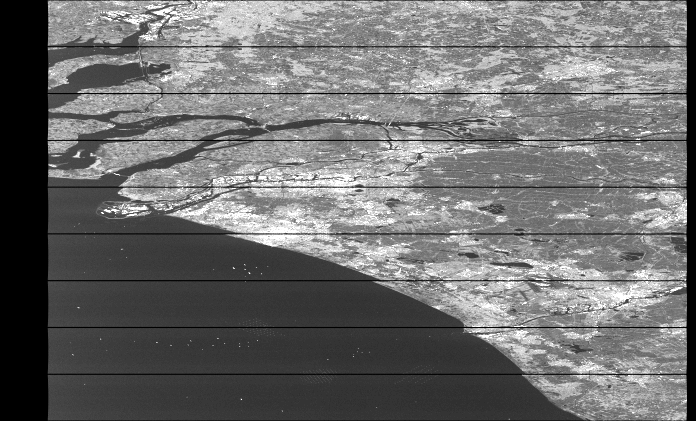
\includegraphics[width=0.5\linewidth]{f/slc_nvh_whole.png}
	\\
	norm(vv iw1) &
	norm(vh iw1)\\
\end{tabular}
\end{frame}

\begin{frame}\ttfamily
AN EXAMPLE RADAR IMAGE: FALSE COLOR\\
===================================\\
$ $\\

1 SLC datum = 6 complex images of size 20.000 x 15.000 \\
	{\color{gray} (vv, vh) x (iw1, iw2, iw3)}\\

	\vfill

	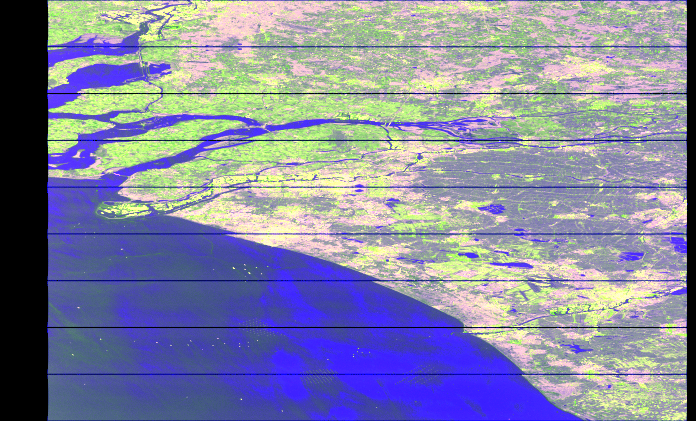
\includegraphics[width=0.8\linewidth]{f/slc_fc_whole.png}\\
	(R, G, B) = (|VH|, |VV|, $\alpha$ |VH|/|VV|)\\
	{\bf only iw1}
\end{frame}

\begin{frame}\ttfamily
AN EXAMPLE RADAR IMAGE: SWATHS\\
==============================\\
$ $\\

	1 SLC datum = 6 complex images of size 20.000 x 15.000 \\
	{\color{gray} (vv, vh) x (iw1, iw2, iw3)}\\

	\vfill

	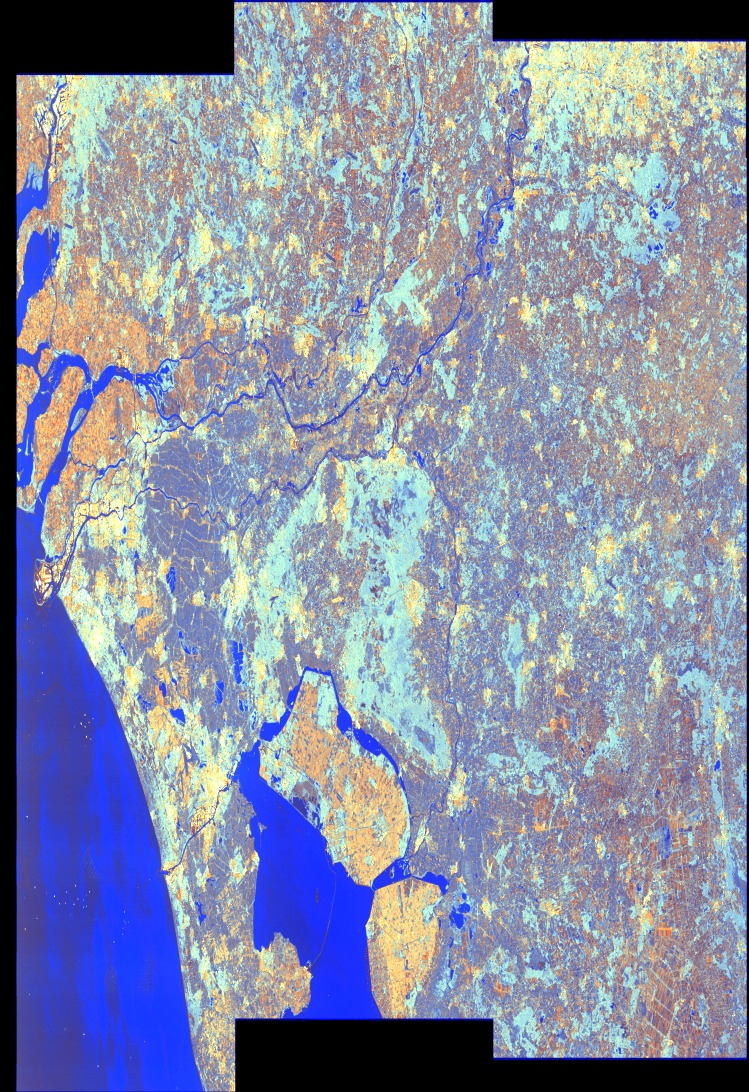
\includegraphics[width=0.4\linewidth]{f/rquick-look.jpg}
	$ $ merging of {\bf iw1, iw2, iw3}
\end{frame}

\begin{frame}\ttfamily
AN EXAMPLE RADAR IMAGE: DETAIL\\
==============================\\
$ $\\

	1 SLC datum = 6 complex images of size 20.000 x 15.000 \\
	{\color{gray} (vv, vh) x (iw1, iw2, iw3)}\\

	\vfill

\begin{tabular}{cc}
	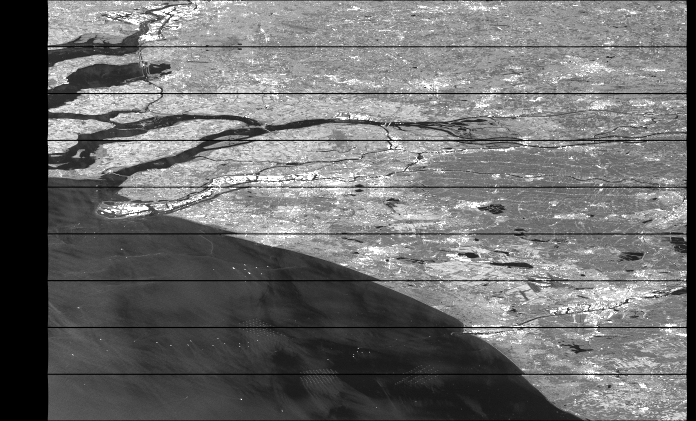
\includegraphics[width=0.5\linewidth]{f/slc_nvv_whole.png}
	&
	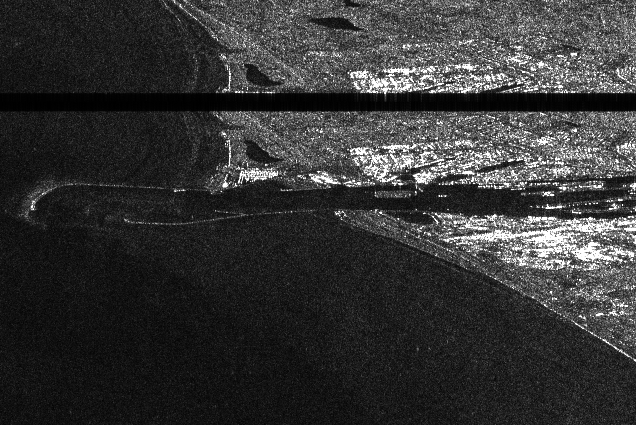
\includegraphics[width=0.5\linewidth]{f/slc_nvv_detail.png}
	\\
	|VV|, whole &
	|VV|, detail 1200x800 \\
\end{tabular}
\end{frame}

\begin{frame}\ttfamily
AN EXAMPLE RADAR IMAGE: COMPLEX NUMBERS\\
=======================================\\
$ $\\


\vfill
	(explore real/imag/angle, RAMPING)

	\vfill\color{darkgray}
	\tiny http://boucantrin.ovh.hw.ipol.im:7788/static/slc/i.html

	\tiny cpu /home/coco/pro/queiroz/phoqueouzygne/data/slc\_vv\_iw2.\%d.tif

	\tiny cpu /home/coco/pro/queiroz/phoqueouzygne/data/nslc\_vv\_iw1.\%d.tif
\end{frame}


\begin{frame}%\ttfamily
%THE BEST INTRODUCTION TO S.A.R. IMAGING\\
%=======================================\\
\vfill
	{\bf Synthetic Aperture Radar: Of Bats and Flying Pianos}\\
	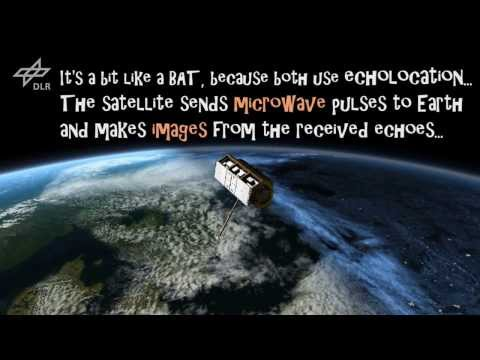
\includegraphics[width=0.9\linewidth]{f/bat.jpg}\\
	{\tt\color{blue} https://www.youtube.com/watch?v=g-YICKbcC-A}
\end{frame}

\begin{frame}\ttfamily
SAR IMAGING: HIGH-LEVEL VIEW\\
============================\\
$ $\\

	\begin{enumerate}
		\item The satellite emits a spherical signal~$f(t)$
		\item The objects in the ground reflect it
		\item The satellite receives the reflected signal~$g(t)$
		\item $I(x,y) = \mathrm{focusing}(g,x,y)$
	\end{enumerate}

	\vfill
	\pause
	\color{red}
	How to create a 2D signal $I(x,y)$ from a 1D signal~$g(t)$ ?
\end{frame}

\begin{frame}\ttfamily
AUDIO SPECTROGRAMS\\
==================\\
$ $\\

	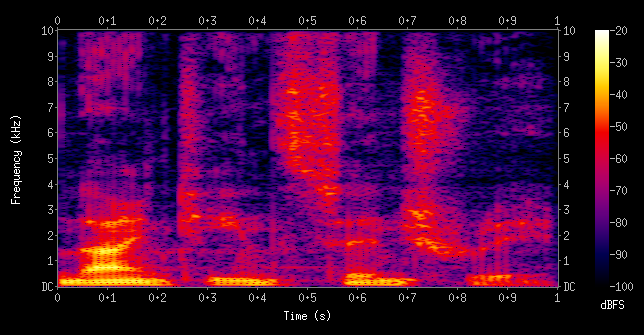
\includegraphics[width=\linewidth]{f/spectrogram.png}\\
	Spectrogram of the spoken words "nineteenth century"

\end{frame}

\begin{frame}\ttfamily
AUDIO SPECTROGRAMS\\
==================\\
$ $\\

	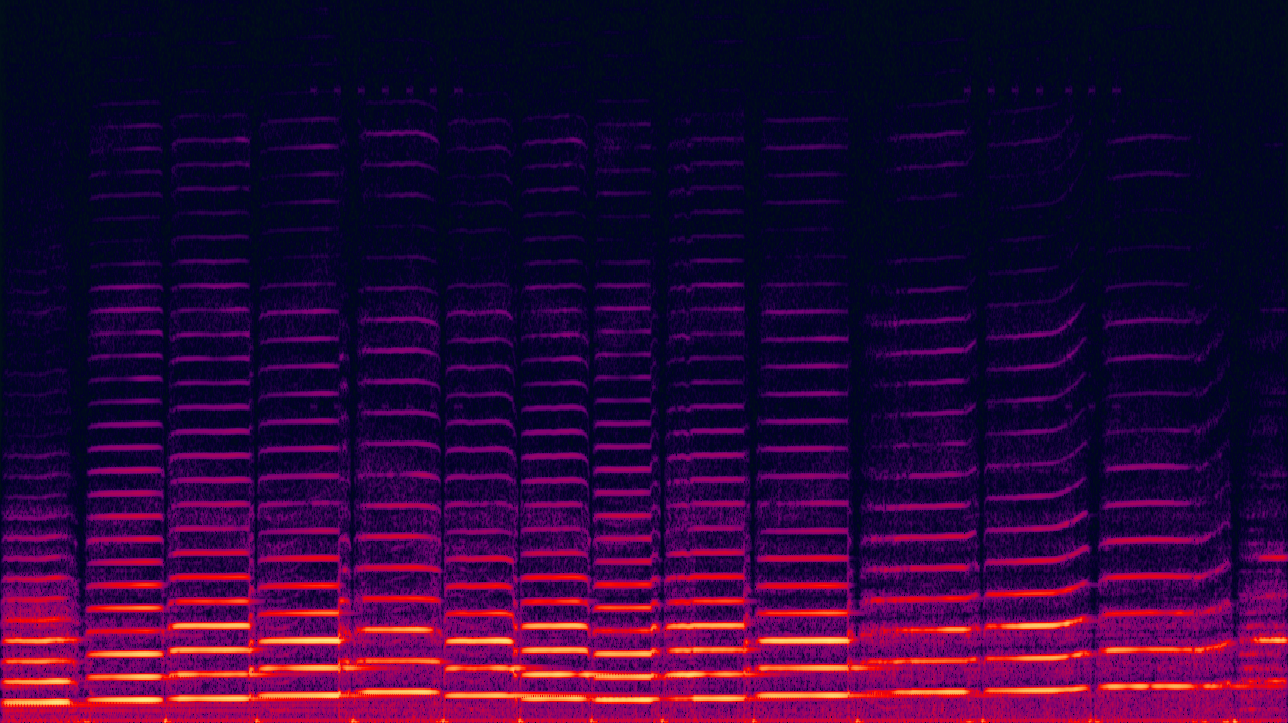
\includegraphics[width=\linewidth]{f/spec_violin.png}\\
	Spectrogram of a violin playing

\end{frame}


\begin{frame}\ttfamily
AUDIO SPECTROGRAMS\\
==================\\
$ $\\

	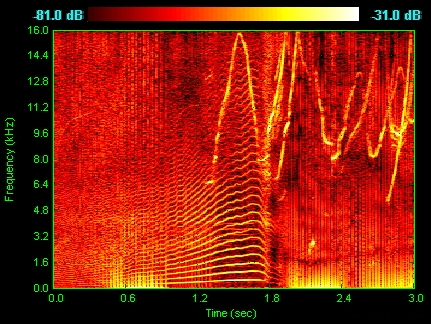
\includegraphics[width=0.7\linewidth]{f/spec_dolphin.jpg}\\
	Spectrogram of a dolphin

\end{frame}

\begin{frame}\ttfamily
GRAVITATIONAL SPECTROGRAMS\\
==========================\\
$ $\\

	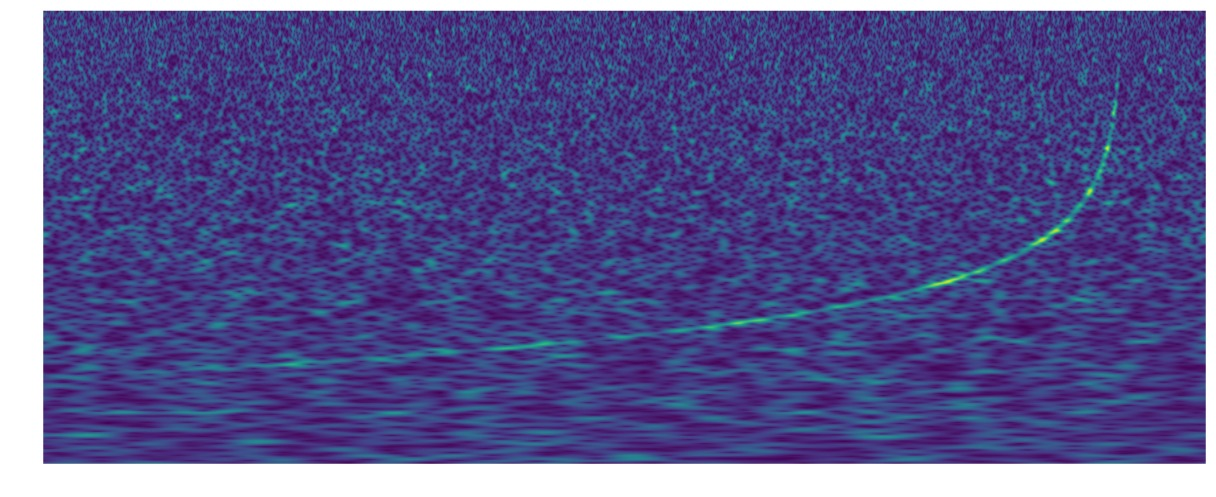
\includegraphics[width=\linewidth]{f/cspec_grav.jpg}\\
	Gravitational Wave {\bf GW170817}

\end{frame}

\begin{frame}\ttfamily
SPECTROGRAM STEGANOGRAPHY\\
=========================\\
$ $\\

	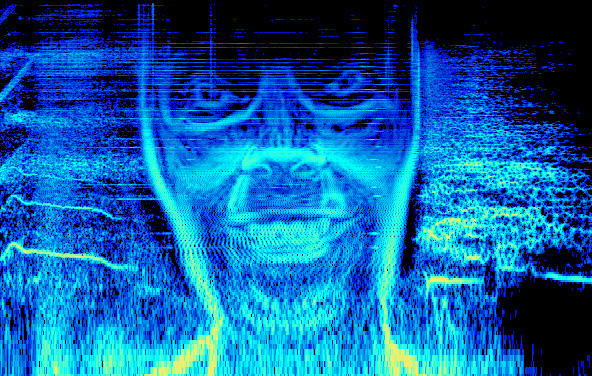
\includegraphics[width=\linewidth]{f/spec_steg.jpg}\\
	Fancy audio spectrogram (hand-edited)

\end{frame}

\begin{frame}\ttfamily
TIME-FREQUENCY ANALYSIS\\
=======================\\
\vfill

	\fbox{
	{\bf Input:} function $x(t)\qquad$ {\bf Output:} function $X(t,f)$
	}

	\vfill

Short-time Fourier transform (e.g., Gabor transform):
	\[
		X(t,f)=\int {\color{blue}w(t-\tau) e^{-if\tau}}x(\tau)\d\tau
		\qquad\qquad \mathrm{avec}\int w = 1
	\]

Wavelet transform:
	\[
		X(t,f)=\int {\color{blue}\frac{1}{\sqrt{f}}\varphi\left(\frac{t-\tau}{f}\right)}x(\tau)\d\tau
		\qquad\qquad \mathrm{avec}\int\varphi = 0
	\]

Wigner transform:
	\[
		X(t,f)=\int {\color{blue}e^{-if\tau}}
		x\left(t+\frac{\tau}{2}\right)
		\widebar{x}\left(t-\frac{\tau}{2}\right)
		\d\tau
	\]

\end{frame}

\begin{frame}\ttfamily
WHAT ARE SAR IMAGES\\
===================\\

\pause
\vfill
SAR images are spectrograms\\
\pause
\vfill


The analysis is performed using a {\color{blue}linear} chirp
	\[
		\color{blue}
		h(t) = \cos(t^2)
	\]
	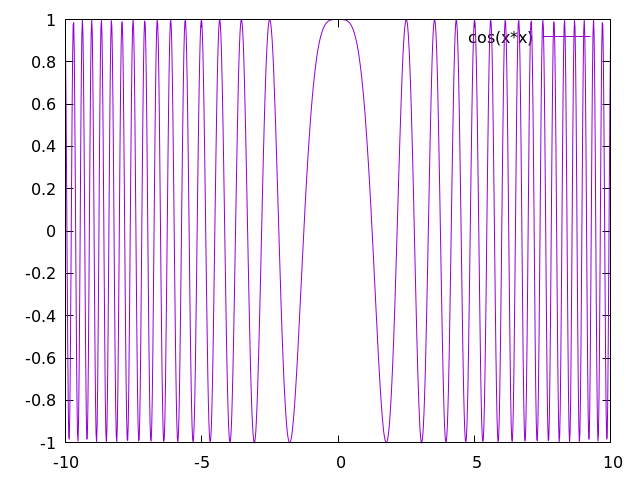
\includegraphics[width=0.6\linewidth]{f/costt.png}
\vfill
	{\scriptsize\color{red}Exercice: why is this function called a linear chirp?}
\end{frame}

\begin{frame}\ttfamily
THE MAGIC OF LINEAR CHIRPS\\
==========================\\
$ $\\

	Let~$h(t)=cos(t^2)$,  numerically, we will have $h\star h = \delta$.
	\vfill\pause

	More precisely, let~$h(t)=\mathrm{rect}\left(\frac{t}{T}\right)e^{iKt^2}$ and~$s_{out}=h\star h$.

	\vfill

	Exact formula:
	\[
		s_{out}(t)=(T-|t|)\mathrm{rect}\left(\frac{t}{2T}\right)
		\mathrm{sinc}\left(Kt(T-|t|)\right)
	\]

	\vfill

	Approximate formula (for $KT^2\ge 100$):
	\[
		s_{out}(t)=
		T\mathrm{sinc}\left(KTt\right)
	\]
\end{frame}

\begin{frame}\ttfamily
PRACTICAL CASE: SENTINEL 1\\
==========================\\
* Sentinel-1: ESA satellite that gives public images\\
* RAW : the received (quantized and encoded) raw data\\
* SLC : complex-valued images, obtained by focusing RAW\\
* GRD : complex-valued images, obtained by resampling SLC
\vfill
	\begin{tabular}{cccc}
		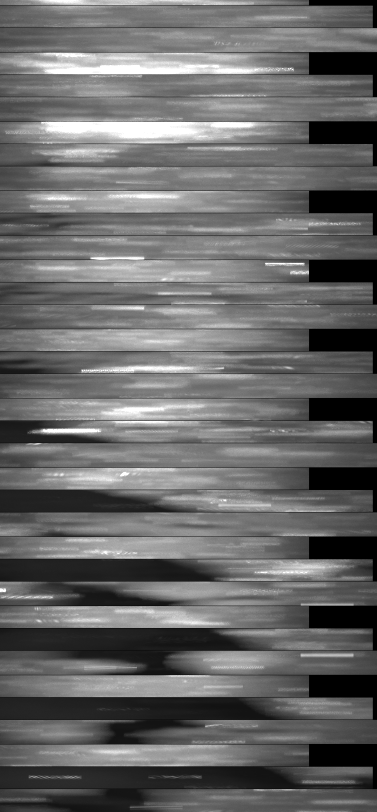
\includegraphics[width=0.23\linewidth]{f/xxx_norm6.png} &
		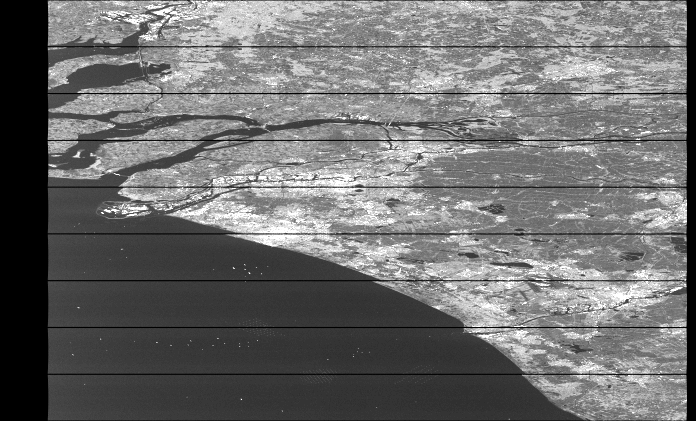
\includegraphics[width=0.23\linewidth]{f/vh5_iw1.png} &
		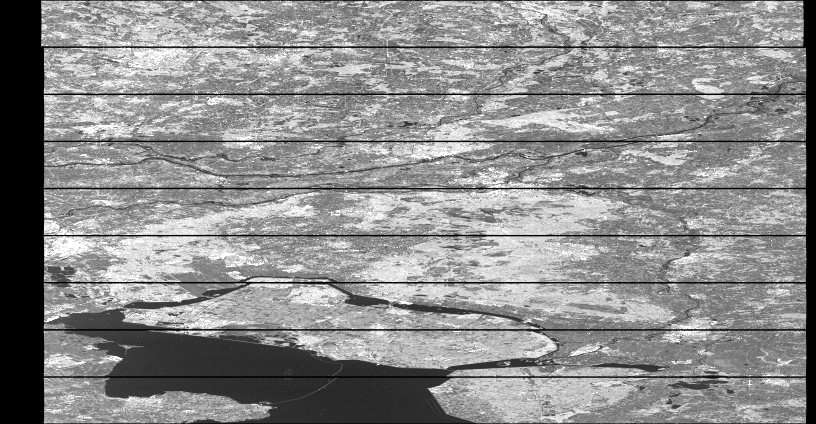
\includegraphics[width=0.23\linewidth]{f/vh5_iw2.png} &
		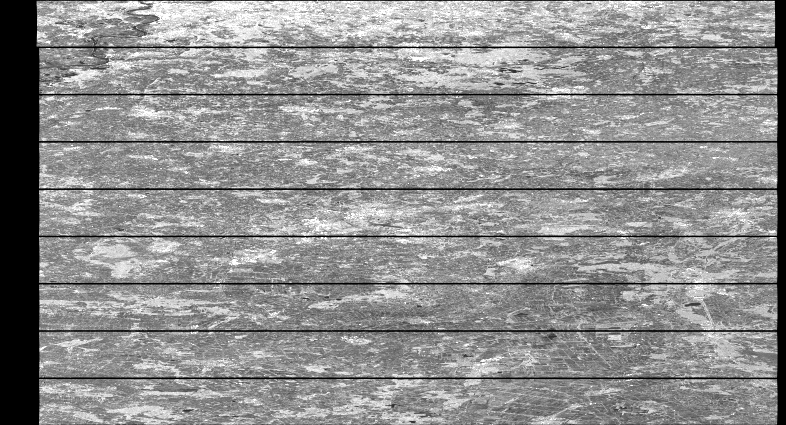
\includegraphics[width=0.23\linewidth]{f/vh5_iw3.png} \\
		\tiny RAW $24076\times51957$ &
		\tiny SLC${}_1$ $22288 \times 13473$ &
		\tiny SLC${}_2$ $26124 \times 13572$ &
		\tiny SLC${}_3$ $25173 \times 13617$ 
	\end{tabular}

\end{frame}

\begin{frame}\ttfamily
	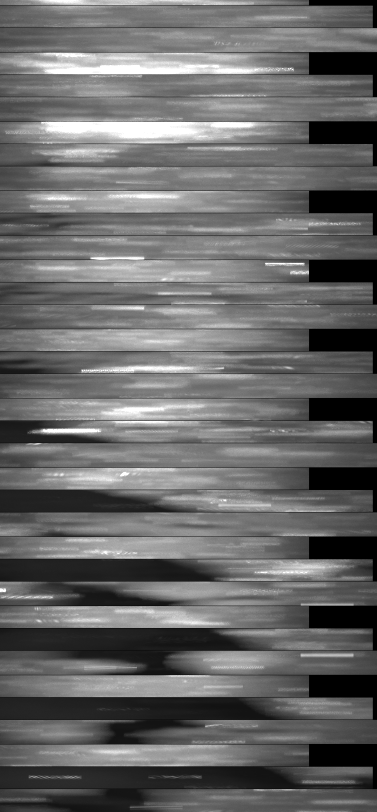
\includegraphics[height=0.99\textheight]{f/xxx_norm6.png}
	$ $
	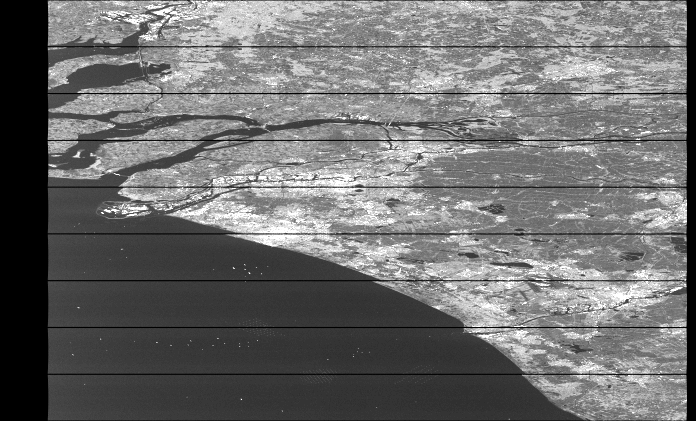
\includegraphics[height=0.4\textheight]{f/vh5_iw1.png}
\end{frame}


\begin{frame}\ttfamily
FOCUSING ALGORITHM\\
==================\\
$ $\\

{\bf Input:} Raw image~$R(x,y)$\\
{\bf Input:} Line range:~$y_a$, $y_b$\\
{\bf Output:} Focused part~$I(x,y)$\\

\begin{enumerate}
	\item Extract relevant lines $C(x,y)$ of~$R(x,y)$.
	\item $T$, $K$, $f$, $\ldots, \leftarrow$ parameters of $C(x,0)$.
	\item Correlate each line with~$h_{K_1,T_1}$
	\item Correlate each column with~$h_{K_2,T_2}$
	\item Output the resulting focused image~$I(x,y)$.
\end{enumerate}

\vfill
\pause
\color{red}
	{\bf Current state of affairs:}~$T_1$ and~$T_2$ are unknown, we estimate their best
values by visual inspection of the final result.

\end{frame}

\begin{frame}\ttfamily
VISUAL EXPLORATION OF FOCUSING PARAMETERS\\
=========================================\\
$ $\\

\vfill
	\color{gray}
	\tiny goto tmux clean ; fpanflip

\end{frame}

\begin{frame}\ttfamily
GOALS AND OPEN PROBLEMS\\
=======================\\
$ $\\

Why do we want to focus ourselves?\\
$\quad$* Intellectual curiosity\\
$\quad$* To focus images on a better-behaved grid\\
$\quad$* To adapt the focusing to a practical problem\\$\quad\ $ (e.g., detection of peaks)\\


\vfill
What is missing?\\
$\quad$* Find the exact parameters in the metadata\\
$\quad$* Understand the tradeoffs of different focusing algos\\
$\quad$* Implementation of the CLEAN algorithm

\vfill

\end{frame}

\end{document}

%%\begin{frame}[plain,fragile]
%%\end{frame}
%%	\ttfamily
%%	\vspace{2em}
%%	{
%%	\centering
%%	{\LARGE FUSION OF IMAGES \\}
%%	\vspace{1em}
%%	}
%%
%%Enric Meinhardt-Llopis\\
%%{\bf SPO} 2018 / 1 / 15
%%	\vfill
%%
%%	% TODO: separte the image into two slides
%
%\begin{frame}\ttfamily
%IMAGE FUSION: TOY EXAMPLE\\
%=========================\\
%\vfill
%%
%%	{\tiny
%	\begin{tabular}{cc}
%		%\includegraphics[width=0.5\linewidth]{ex1/s_lletja_111.png} &
%		\animategraphics[width=0.5\linewidth,loop,autoplay]{4}{ex1/s_lletja_}{100}{149} &
%		\includegraphics[width=0.5\linewidth]{ex1/isamarkand.png} \\
%		input &
%		output \\
%	\end{tabular}
%%	}
%\end{frame}
%
%%\begin{frame}[plain]
%%	\includegraphics[height=\textheight]{f/cigares.png}
%%\end{frame}
%
%
%\begin{frame}\ttfamily
%GENERAL PROBLEM\\
%===============\\
%
%	%An image is a function~$\R^2\to\R^d$, with $d=1$ or $d=3$.
%
%	Given a list of distorted images %$\A_i:\R^2\to\R^d$ %for~$i=1,\ldots,N$
%\[
%	{\color{red}A_i}(x)
%	=
%	\only<1>{{\color{blue}A} (x) + n_i(x)}
%	\only<2>{{\color{blue}A} (x) + b_i(x) + n_i(x)}
%	\only<3>{{\color{blue}A} (x + \varphi_i(x)) + b_i(x) + n_i(x)}
%	\only<4>{k_i * {\color{blue}A} (x + \varphi_i(x)) + b_i(x) + n_i(x)}
%	\only<5>{M_i\cdot\left[ k_i * {\color{blue}A} (x + \varphi_i(x)) + b_i(x) + n_i(x) \right]}
%	\qquad
%	\qquad
%	i=1,\ldots,N
%\]
%we want to recover the {\bf latent image}~${\color{blue}A}(x)$.
%
%\vfill
%
%Where
%
%\bigskip
%
%\begin{tabular}{ll}
%	$n_i$ & additive noise fields (white noise) \\
%	\uncover<2->{$b_i$ & additive bias fields (piecewise smooth)} \\
%	\uncover<3->{$\varphi_i$ & deformation fields} \\
%	\uncover<4->{$k_i$ & blur kernels} \\
%	\uncover<5->{$M_i$ & binary masks} \\
%\end{tabular}
%
%\end{frame}
%
%
%
%\begin{frame}[fragile]\begin{verbatim}
%CONTENTS
%========
%
%
%0. Gallery of applications
%
%1. Image fusion in the spatial domain
%
%2. Image fusion in the frequency domain
%
%3. Dual-domain fusion (open problem)
%\end{verbatim}
%\end{frame}
%
%
%\begin{frame}\tt
%APPLICATIONS OF IMAGE FUSION : DENOISING\\
%========================================\\
%
%	\begin{tabular}{cc}
%		\includegraphics[width=0.5\linewidth]{f/igstatue_crop.png}&
%		\includegraphics[width=0.5\linewidth]{f/igstatue_crop_denoised.png}\\
%		$A_1(x)$ &
%		$\displaystyle\frac{A_1(x)+\cdots+A_{10}(x)}{10}$
%		%\small image 1/10 &
%		%\small pointwise average of the 10 \\
%	\end{tabular}
%\end{frame}
%
%
%\begin{frame}\tt
%APPLICATIONS OF IMAGE FUSION : MUSEUM PHOTOGRAPHY\\
%=================================================\\
%
%\vfill
%
%\begin{tabular}{cccc}
%	\includegraphics[height=0.52\textheight]{slcon3/clave/cy04.png}&
%	\includegraphics[height=0.52\textheight]{slcon3/clave/cy05.png}&
%	\includegraphics[height=0.52\textheight]{slcon3/clave/Rmed.jpg}&
%	\includegraphics[height=0.52\textheight]{slcon3/clave/diff5.jpg}\\
%	$A_3$ &
%	$A_5$ &
%	$B = {\color{red}f}(\{A_i\})$ &
%	$A_5\circ\varphi_5-B$
%	%in$_3$ &
%	%in$_5$ &
%	%out &
%	%diff$_5$
%\end{tabular}
%
%\vfill
%
%\end{frame}
%
%
%\begin{frame}\tt
%APPLICATIONS OF IMAGE FUSION : VIRTUAL PERISCOPE\\
%================================================\\
%
%\vfill
%
%	\begin{tabular}{cc}
%		\includegraphics[width=0.5\textwidth]{pedf/phua/fhu/submarine.png} &
%		\includegraphics[width=0.5\textwidth]{pedf/phua/fhu/submarinev.png} \\
%		Regular Periscope &
%		Virtual Periscope \\
%	\end{tabular}
%
%	\vfill
%
%	{\bf Problem:} how to process these images?
%\end{frame}
%
%\begin{frame}\tt
%APPLICATIONS OF IMAGE FUSION : VIRTUAL PERISCOPE\\
%================================================
%
%\bigskip
%\tiny
%	\animategraphics[width=0.9\linewidth,loop,autoplay]{10}{pedf/phua/f3/cosa-000}{01}{32}
%
%	{\color{gray}
%		Video sequence courtesy of Y.Y.~Schechner
%		and M.~Alterman, Technion, Israel
%	}
%\end{frame}
%
%\begin{frame}\tt
%APPLICATIONS OF IMAGE FUSION : VIRTUAL PERISCOPE
%%================================================
%
%\begin{overlayarea}{\textwidth}{0.9\textheight}
%	\vfill
%\only<1>{\includegraphics[width=0.9\textwidth]{pedf/phua/f3/cosa-00011.png}\\frame 11/35}%
%\only<2>{\includegraphics[width=0.9\textwidth]{pedf/phua/f3/avg_orig.png}\\average of  35 video frames}%
%\only<3>{\includegraphics[width=0.9\textwidth]{pedf/phua/f3/weisz_QQ.png}\\our reconstruction from 35 video frames}%
%\end{overlayarea}
%\end{frame}
%
%\begin{frame}\tt
%APPLICATIONS OF IMAGE FUSION : ASTRONOMICAL SEEING\\
%==================================================\\
%
%
%\scriptsize
%	\begin{tabular}{lll}
%		\includegraphics[width=0.25\linewidth]{f/lucky_bad.png} &
%		\includegraphics[width=0.25\linewidth]{f/lucky_good.png} &
%		\pause
%		\includegraphics[width=0.25\linewidth]{f/lucky_avg.png} \\
%		bad frame &
%		good frame &
%		average of all \\
%		& & \\
%		\includegraphics[width=0.25\linewidth]{f/lucky_avg_50.png} &
%		\includegraphics[width=0.25\linewidth]{f/lucky_avg_r50.png} &
%		\includegraphics[width=0.25\linewidth]{f/lucky_avg_r25.png} \\
%		reg. avg of all &
%		reg. avg of 50\% best &
%		reg. avg of 25\% best \\
%	\end{tabular}
%
%	\vfill
%	\color{gray}
%	[Hippler et al.,
%	The AstraLux Sur Lucky Imaging Instrument at the NTT,\\
%	The ESO Messenger 137 (2009)]
%
%\end{frame}
%
%\begin{frame}\tt
%APPLICATIONS : ASTEROID 3D RECONSTRUCTION\\
%==========================================\\
%
%\animategraphics[width=0.9\linewidth,loop,autoplay]{2}{f/lute_}{1}{2}
%
%\scriptsize
%	Images of asteroid 21 Lutetia taken by the ROSETTA spaceship (ESA)
%\end{frame}
%
%\begin{frame}\tt
%APPLICATIONS : ASTEROID 3D RECONSTRUCTION\\
%==========================================\\
%
%
%\vfill
%\hspace*{1pt}\makebox[\linewidth][c]{%
%	\small\begin{tabular}{ll}
%		\includegraphics[width=0.56\linewidth]{f/lutetia_both.jpg}&
%		\includegraphics[width=0.55\linewidth]{f/lutetia_gold.jpg}\\
%		Yellow: shape from parallax&
%		fusion of frequencies \\
%		White: shape from shading &\\
%	\end{tabular}
%	}
%\vfill
%
%\end{frame}
%
%
%
%\begin{frame}\tt
%APPLICATIONS : CAMERA SHAKE DEBLURRING\\
%======================================\\
%
%	\includegraphics[width=\linewidth]{f/shakeblur.jpg}
%
%	M.Delbracio, G.Sapiro,
%	{\it Removing Camera Shake via Weighted Fourier Burst Accumulation},
%	2015
%\end{frame}
%
%
%%\begin{frame}\tt
%%APPLICATIONS : LIDAR POINT CLOUD COLORIZATION\\
%%=============================================\\
%%
%%\end{frame}
%
%
%%\begin{frame}\tt
%%APPLICATIONS : TEXTURE SYNTHESIS\\
%%================================\\
%%
%%\end{frame}
%
%
%\begin{frame}\tt
%APPLICATIONS : IMAGE STITCHING\\
%==============================\\
%
%\scriptsize
%	\includegraphics[width=\linewidth]{f/stitching_process.jpg}
%
%	Katherine A.Scott, Fish-Eye Lens Dewarping and Panorama Stitching, 2013
%\end{frame}
%
%
%\begin{frame}\tt
%APPLICATIONS : TRAFFIC TICKETS FROM OUTER SPACE\\
%===============================================\\
%
%\vfill
%
%\footnotesize
%\begin{tabular}{ll}
%	\includegraphics[width=0.48\textwidth]{grisifi/f/rgb_before.png}&
%	\includegraphics[width=0.48\textwidth]{grisifi/f/output.png}\\
%	{\bf input:} {\it one} multispectral image &
%	{\bf output:} speed of cars in the road
%\end{tabular}
%\vfill
%
%\end{frame}
%
%
%\begin{frame}\tt
%APPLICATIONS : TRAFFIC TICKETS FROM OUTER SPACE\\
%===============================================\\
%
%
%\only<1>{\includegraphics[width=0.7\textwidth]{grisifi/f/boulogne_sentinel.png}}%
%\only<2>{\includegraphics[width=0.7\textwidth]{grisifi/f/boulogne_wv3_msi.png}}%
%\only<3>{\includegraphics[width=0.7\textwidth]{grisifi/f/boulogne_wv3_pan.png}}
%
%\end{frame}
%
%%\begin{frame}\tt
%%APPLICATIONS : DETECTION OF TREES IN D.S.M.\\
%%===========================================\\
%%
%%\end{frame}
%
%
%\begin{frame}\tt
%THE EMPEROR'S NOSE PARADOX (FEYNMAN, JAYNES, ...)\\
%=================================================\\
%
%
%The empire has 1.000.000.000 people.  Each person knows the size of the
%emperor's nose with an error less than 1~meter.  By computing the average
%of these observations, we obtain an error smaller than
%\[
%	1m\cdot\frac{1}{\sqrt{1.000.000.000}} = 0.0316mm
%\]
%
%\vfill\pause
%	{\bf Is image fusion hopeless, in general?}
%
%\end{frame}
%
%\begin{frame}\tt
%THE MONA LISA EXPERIMENT\\
%========================\\
%
%1. Search "mona lisa" on google images\\
%2. Download the first~$N=1000$ results\\
%3. Apply your best image fusion algorithm\\
%
%\pause
%Can you obtain a perfect rendering of the painting?\\
%\pause
%\includegraphics[width=\linewidth]{f/louvre.jpg}
%\end{frame}
%
%
%
%\begin{frame}[fragile]\tt%\begin{verbatim}
%CONTENTS\\
%========\\
%$ $\\
%
%1. Image fusion in the spatial domain\\
%
%1.0. Crash course in accumulators: means, medians, modes\\
%1.1. Pointwise fusion using accumulators\\
%1.2. Registration + fusion {\color{gray}(and the centroid method)}\\
%1.3. Weighted fusion {\color{gray}(and lucky frames)}\\
%1.4. PDE-based fusion\\
%%\end{verbatim}
%%1.5. Long-term goal: mona lisa, unfulfilled
%\end{frame}
%
%
%
%\begin{frame}\tt
%CRASH COURSE IN ACCUMULATORS : BIBLIOGRAPHY\\
%===========================================\\
%
%\scriptsize
%	\includegraphics[height=0.8\textheight]{f/bullen.jpg}
%	$\ $ 538 pages (summary in the next 4 slides)
%
%\end{frame}
%
%\begin{frame}\tt
%THE CLASSICAL ``MEANS''\\
%=======================
%
%\vfill
%
%	Given~$N$ {\color{red} positive} numbers~$x_1,\ldots, x_N$, define
%	\begin{eqnarray*}
%		\mathrm{avg} & :=& ({x_1+\cdots+x_N})/{N} \\
%		\mathrm{geo} & :=& \sqrt[N]{x_1\cdot \cdots\cdot x_N} \\
%		\mathrm{har} & :=& {N}/({{1}/{x_1}+\cdots+{1}/{x_N})} \\
%		\mathrm{cha} & :=& {(x_1^2+\cdots+x_N^2)}/({x_1+\cdots+x_N}) \\
%		\mathrm{rms} & :=& \sqrt{(x_1^2+\cdots+x_N^2)/{N}} \\
%%		\mathrm{med} & :=& x_{(N/2)}
%	\end{eqnarray*}
%%	where $x_{(1)}, \ldots, x_{(N)}$ are the sorted input numbers.
%	\vfill
%
%Fundamental inequality:
%\[
%	\mathrm{min}
%	\le \mathrm{har}
%	\le \mathrm{geo}
%	\le \mathrm{avg}
%	\le \mathrm{rms}
%	\le \mathrm{cha}
%	\le \mathrm{max}
%\]
%
%\end{frame}
%
%\begin{frame}\tt
%THE POWER MEANS $M_p$\\
%=====================
%
%\[
%	M_p := \sqrt[p]{\frac{x_1^p+\cdots+x_N^p}{N}}
%\]
%
%\pause
%
%\vfill
%
%Particular cases (taking limits if necessary):
%
%\vfill
%
%\begin{tabular}{c|c}
%	power mean & meaning \\
%	\hline
%	$M_{-\infty}$ & minimum \\
%	$M_{-1}$ & harmonic mean \\
%	$M_0$ & geometric mean \\
%	$M_1$ & arithmetic mean \\
%	$M_2$ & quadratic mean \\
%	$M_3$ & cubic mean \\
%	$M_\infty$ & maximum \\
%\end{tabular}
%\end{frame}
%
%\begin{frame}\tt
%LEHMER~$L_p$ MEANS\\
%===============
%
%%Lehmer means
%\[
%	L_p(x_1,\ldots,x_N):=\frac{
%%		\displaystyle\sum_{i=1}^N x_i^p
%		x_1^p +\cdots+x_N^p
%		}{
%%		\displaystyle\sum_{i=1}^N x_i^{p-1}
%			x_1^{p-1} +\cdots+x_N^{p-1}
%		}
%\]
%
%\begin{tabular}{l|l}
%	Lehmer mean & name \\
%	\hline
%	$L_{-\infty}$ & min \\
%	$L_0$ & harmonic \\
%	$L_{0.5}$ & geometric  (for $N=2$)\\
%	$L_1$ & arithmetic \\
%	$L_2$ & counterharmonic 
%	$(x_1^2+\cdots+x_N^2)/(x_1+\cdots+x_N)$ \\
%	$L_{\infty}$ & max \\
%\end{tabular}
%\end{frame}
%
%\begin{frame}\tt
%GINI~$G_{p,q}$ MEANS\\
%===============
%
%%Gini means
%\[
%	G_{p,q}(x_1,\ldots,x_N) :=
%	\begin{cases}
%		\sqrt[p-q]{\displaystyle\frac{\sum x^p}{\sum x^q}}
%		& \textrm{if}\ p\neq q \\
%		&\\
%		\sqrt[\sum x^p]{\prod x^{x^p}}
%		& \textrm{if}\ p=q
%	\end{cases}
%\]
%where the sums and products above are performed over~$x\in\{x_1,\ldots
%x_N\}$
%
%\vfill
%
%Particular cases:\\
%	$\qquad L_p = G_{p,p-1}$\\
%	$\qquad M_p = G_{p,0}$\\
%
%\pause
%
%{\bf Observation:} the ``handbook of means'' deals mostly with Gini means and
%	their inequalities, and with more general means of two numbers, always
%	positive.\\{\color{red}The words ``median'' and ``mode'' do not appear}.
%
%\end{frame}
%
%\begin{frame}\tt
%AXIOMS FOR ACCUMULATORS $f:\R^N\to\R$\\
%==================================
%
%%A map~$f:\R^N\to\R$ can have the following properties
%\vfill
%%is called an aggregator function:
%\begin{itemize}
%	\item[S1.]
%		(Symmetry)
%		$\quad$
%		$f(x_{\sigma_1},\ldots,x_{\sigma_N})=f(x_1,\ldots,x_N)
%		\quad
%		\forall\sigma\in\mathrm{S}_N$
%	\item[S2.]
%		(Reflexivity)
%		$\qquad$
%		$f(c,\ldots,c)=c$
%	\item[S3.]
%		(Composability)
%		$\ $
%		$f\left(f(x_1,\ldots,x_P),\ldots,f(x_{P(Q-1)},\ldots,x_{PQ})\right)
%		=f(x_1,\ldots,x_N)\quad\forall PQ=N$
%\end{itemize}
%\begin{itemize}
%	\item[T1.]
%		(Monotony)
%		$\quad$
%		%$(x_1,\ldots,x_N)\le(y_1,\ldots,y_N)
%		%\implies
%		%f(x_1,\ldots,x_N)\le f(y_1,\ldots,y_N)$
%		$(\x)\le(\y)
%		\implies
%		f(\x)\le f(\y)$
%	\item[T2.]
%		(Bracketing)
%		$\quad$
%		%$\mathrm{min}(x_1,\ldots,x_N)
%		%\le f(x_1,\ldots,x_N)
%		%\le \mathrm{max}(x_1,\ldots,x_N)$
%		$\mathrm{min}(\x)
%		\le f(\x )
%		\le \mathrm{max}(\x)$
%	\item[T3.]
%		(Continuity)
%		$\qquad$
%		$f:\R^N\to\R$ is continuous
%\end{itemize}
%\begin{itemize}
%	\item[A1.]
%		(Homogeneity)
%		$\ $
%		$f(\lambda x_1,\ldots,\lambda x_N)
%		=\lambda\ f(x_1,\ldots,x_N)
%		%\quad\forall\lambda >0
%		$
%	\item[A2.]
%		(Shift)
%		$\quad$
%		$f(\lambda+x_1,\ldots,\lambda+x_N)
%		=\lambda+f(x_1,\ldots,x_N)$
%	\item[A3.]
%		(Additivity)
%		$\quad$
%		$f(\x+\y)=f(\x) + f(\y)$
%\end{itemize}
%
%\end{frame}
%
%
%\begin{frame}\tt
%ORDER STATISTICS $O_k$ and $U_\alpha$\\
%=====================================
%
%	\[
%	O_k(x_1,\ldots,x_N) := x_{(k)}\qquad k=1,\ldots,N
%	\]
%
%
%	\[
%		U_\alpha(x_1,\ldots,x_N) :=\  ''\!x_{((N-1)\alpha+1)}{}''\qquad \alpha\in[0,1]
%	\]
%(with linear interpolation between neighboring points)
%
%	\vfill
%
%	%Particular cases:
%
%
%\begin{tabular}{l|l}
%	order statistic & meaning \\
%	\hline
%	$U_0$ & minimum \\
%	$U_{0.1}$ & first decile \\
%	$U_{0.25}$ & first quartile \\
%	$U_{0.5}$ & median \\
%	$U_{0.75}$ & third quartile \\
%	$U_{0.9}$ & ninth decile \\
%	$U_1$ & maximum \\
%\end{tabular}
%\end{frame}
%
%\begin{frame}\tt
%L-ESTIMATORS AND $I_\alpha$\\
%===================
%
%Interpolation between min and max
%\[
%	I_{\alpha}:=\alpha U_1 + (1-\alpha) U_0
%\]
%
%General case: convex combination of order statistics
%\[
%	L := \frac{\sum_{k=1}^N{\alpha_kO_k}}{\sum_{k=1}^N{\alpha_k}}
%\]
%
%\begin{tabular}{l|l}
%	$L$-estimator & name \\
%	\hline
%	$U_0$ & min \\
%	$U_1$ & max \\
%	$(U_0+U_1)/2$ & midrange \\
%	$(U_{0.25}+U_{0.75})/2$ & midhinge (avg. of quartiles) \\
%	$(U_{0.25}+2U_{0.5}+U_{0.75})/4$ & trimean (avg. of median
%	and midhinge) \\
%	$\frac{2}{N}\sum_{k>N/4}^{3N/4} U_k$ & midmean (avg. of
%	central half) \\
%	$\frac{1}{N}\sum_{k=1}^{N} U_k$ & mean (avg. of
%	everything)
%\end{tabular}
%\end{frame}
%
%\begin{frame}\tt
%L-ESTIMATORS\\
%============
%
%\vfill
%
%
%An advantage of the trimean as a measure of the center (of a
%distribution) is that it combines the median's emphasis on center
%values with the midhinge's attention to the extremes.\hfill
%
%
%\vfill
%
%	---Herbert F. Weisberg,\\ \emph{Central Tendency and Variability}
%\vfill
%\end{frame}
%
%\begin{frame}\tt
%HISTOGRAM MODES $H_{\varphi,\psi}$\\
%====================\\
%
%Discrete case:\\
%Mode = number that appears more times.
%
%\bigskip
%
%The continuous case is reduced to the discrete by quantization, using a bin size~$\varphi$ and
%	a bin offset~$\psi$:
%
%\[
%	H_{\varphi,\psi}(x_1,\ldots,x_N) :=
%	\psi+\frac{1}{2}\varphi+\varphi\argmax_{k\in\Z}
%%	\sum_{i=1}^N\int_0^1
%%	\delta\left(y+k+\frac{\psi-x_i}{\varphi}\right)\d y
%	\sum_{i=1}^N\int_{\psi+k\varphi}^{\psi+(k+1)\varphi}
%	\delta(x-x_i)\,\d x
%\]
%(center of the bin with most samples)
%
%\vfill
%
%	\pause\color{red}
%	Observation: the dependence on $(\varphi,\psi)$ is FRACTAL
%
%\vfill
%
%\end{frame}
%
%\begin{frame}\tt
%THE HISTOGRAM FRACTAL: $H_{\varphi,\psi}$ of 100 normal deviates\\
%===================================================
%
%\includegraphics[width=\linewidth]{f/histofractal.png}
%
%\end{frame}
%
%\begin{frame}\tt
%FRECHET $p$-CENTROIDS $F_p$\\
%======================
%
%Fréchet centroid of points~$p_i$ on a metric space:
%\[
%	c := \argmin_{m\in\R}\sum_{i=1}^N d^2(p_i,m).
%\]
%
%Fréchet $p$-centroid of~$N$ real numbers:
%\[
%	F_p(x_1,\ldots,x_N) :=
%	\argmin_{m\in\R}\sqrt[p]{\frac{1}{N}\sum_{i=1}^N|x_i-m|^p}
%\]
%
%\pause
%
%\begin{tabular}{l|l}
%	Fréchet centroid & meaning \\
%	\hline
%	$F_2$ & average \\
%	$F_1$ & median \\
%	$F_{\to0}$ & ``continuous mode'' \\
%	$F_{\to\infty}$ & midrange $I_{0.5}=(\min+\max)/2$ \\
%	$F_{0.5}$ & {\it soft mode} \\
%\end{tabular}
%\end{frame}
%
%
%\begin{frame}\tt
%CRASH COURSE ON ACCUMULATORS : CONCLUSION\\
%=========================================\\
%
%The best accumulators are the Fréchet p-centroids
%\[
%	F_p(x_1,\ldots,x_N) :=
%	\argmin_{m\in\R}\sum_{i=1}^N|x_i-m|^p
%\]
%
%	(1) They are shift-invariant (as opposed to all cases of Gini means except the average).\\
%
%	(2) The definition extends directly to negative numbers and vectors
%	\uncover<2->{{\color{blue}and can admit weights}}
%\[
%	\only<1>{F_p(\vec x_1,\ldots,\vec x_N) :=
%\argmin_{\vec m\in\R^d}\sum_{i=1}^N\|\vec x_i-\vec m\|^p}
%	\only<2>{F_p(\vec x_1,\ldots,\vec x_N,{\color{blue}w_i}) :=
%\argmin_{\vec m\in\R^d}\sum_{i=1}^N{\color{blue}w_i}\|\vec x_i-\vec m\|^p}
%\]
%
%	\color{gray}
%Particular cases: $F_1$=average, $F_2$=median,
%	$F_0$=mode (!), $F_\infty$=barycenter of convex hull.
%
%\end{frame}
%
%\begin{frame}\tt
%OPEN PROBLEM ?\\
%==============\\
%
%If~$p<1$, can you compute
%	\[
%	F_p(\vec x_1,\ldots,\vec x_N) :=
%	\argmin_{\vec m\in\R^d}\sum_{i=1}^N\|\vec x_i-\vec m\|^p
%\]
%	in time~$O(N)$ ?\pause
%
%	$\ $
%
%
%	{\color{gray}( the naive algorithm for $d=1$ takes~$O(N^2)$ )}
%
%	$\ $
%
%	$\ $
%
%	The answer is probably yes;
%	for~$d=1$, there are some easy heuristics to try,
%	but I do not know any algorithm.
%\end{frame}
%
%%1.1. Pointwise fusion using accumulators\\
%%1.2. Registration + fusion {\color{gray}(and the centroid method)}\\
%%1.3. Weighted fusion {\color{gray}(and lucky frames)}\\
%%1.4. PDE-based fusion\\
%
%
%\begin{frame}\tt
%POINTWISE FUSION USING ACCUMULATORS\\
%===================================\\
%
%	Given an accumulator function~$\color{red}f$, we can do image fusion:\\
%
%
%	{\bf Input:} $\ \ A_i(x)\qquad i=1,\ldots,N$\\
%	{\bf Output:} $B(x) = {\color{red}f}(A_1(x), \ldots, A_N(x))$\\
%
%	\begin{tabular}{ccccc}
%		\animategraphics[width=0.18\linewidth,loop,autoplay]{5}{slcon3/clave/pRi}{00}{05} &
%		\includegraphics[width=0.18\linewidth]{slcon3/clave/fp_min.png}&
%		\includegraphics[width=0.18\linewidth]{slcon3/clave/fp_avg.png}&
%		\includegraphics[width=0.18\linewidth]{slcon3/clave/fp_med.png}&
%		\includegraphics[width=0.18\linewidth]{slcon3/clave/fp_max.png}\\
%		$A_i$ &
%		$f=\mathrm{min}$ &
%		$f=\mathrm{avg}$ &
%		$f=\mathrm{med}$ &
%		$f=\mathrm{max}$ \\
%	\end{tabular}
%
%	\vfill\pause\color{gray}
%	{\bf Conclusion:} The median is better, but not perfect
%
%\end{frame}
%
%\begin{frame}\tt
%GENERIC FUSION ALGORITHM (REGISTRATION + ACCUMULATION)\\
%======================================================\\
%
%
%	{\bf Input:} Images $\ A_i(x)\quad i=1,\ldots,N$\\
%	{\bf Output:} Image $B(x)$\\
%	{\bf Algorithm:}\\
%	1. Select a ``centered'' reference image ~$r\in\{1,\ldots,N\}$\\
%	2. Find~$\varphi_i$ s.t.~$A_i\circ\varphi_i\approx A_r$ (registration)\\
%	3. $B(x):=f(\ A_1(\varphi_1(x)),\ \ldots,\ A_N(\varphi_N(x))\ )$\\
%
%	\pause
%	{\bf Analysis:}
%\begin{itemize}
%	\item[{\color{darkgreen}\Checkmark}] It may invert the model
%		$A_i(x) = A(\varphi_i(x))+n_i(x)$
%	\item[{\color{darkgreen}\Checkmark}] Good results when~$\varphi_i\approx\mathrm{id}$ and~$n_i\approx 0$
%	\item[{\color{red}\XSolidBrush}] The $\varphi_i$ are difficult to estimate when~$n$ is large
%	\item[{\color{red}\XSolidBrush}] Accumulators often fail with few images (e.g. N=3)
%		\pause
%	\item[{\color{red}\XSolidBrush}] WHAT IF NONE OF THE IMAGES IS ``CENTERED''?
%\end{itemize}
%
%\end{frame}
%
%\begin{frame}\tt
%POINTWISE FUSION WITHOUT A REFERENCE IMAGE\\
%==========================================\\
%
%\animategraphics[width=0.6\linewidth,loop,autoplay]{10}{pedf/pdescartes/f3/samarkand_30_5_}{1000}{1019}
%
%\small
%Any reference image from this sequence will be ``wobbly''.  Can we recover a
%	``straight'' image ?  It seems impossible, but...
%
%\end{frame}
%
%
%\begin{frame}
%	\frametitle{Géomètrie du Flot Optique}
%
%	Le flot optique est une diréction tangente à la sous-varieté des images
%	nettes (en rouge, ci-dessus).
%	\vfill
%
%	\includegraphics[width=\textwidth]{pedf/pdescartes/f1/geomflow.png}
%\end{frame}
%
%\begin{frame}
%	\frametitle{Propriétés du flot optique}
%	Le flot optique permet d'interpoler images sans inventer de nouvelles
%	couleurs.
%	\vfill
%
%	%FIGs: faces
%	\begin{tabular}{cccc}
%		\includegraphics[width=0.2\textwidth]{pedf/pdescartes/f/psad.png} &
%		\includegraphics[width=0.2\textwidth]{pedf/pdescartes/f/phappy.png} &
%		\only<1>{\includegraphics[width=0.2\textwidth]{pedf/pdescartes/f/psum.png}}\only<2>{\includegraphics[width=0.2\textwidth]{pedf/pdescartes/f/plmix25.png}} &
%		\only<1>{\includegraphics[width=0.2\textwidth]{pedf/pdescartes/f/pnormal.png}}\only<2>{\includegraphics[width=0.2\textwidth]{pedf/pdescartes/f/pmix25.png}} \\
%		$A$ & $B$ & $A+\frac{1}{\only<1>{2}\only<2>{4}}(B-A)$ &
%		$A\boxplus\frac{1}{\only<1>{2}\only<2>{4}}F_{AB}$ \\
%	\end{tabular}
%
%	\vfill
%	{\footnotesize Notation:\\Si~$\varphi=\mathrm{Id}+\u$ est un
%	difféomorphisme du plan, alors~$A\circ\varphi^{-1}$ est
%	noté~$A\boxplus\u$}
%\end{frame}
%
%\begin{frame}
%	\frametitle{Correction de la turbulence par flot optique}
%	{\bf Idée:} au lieu de moyenner les images, moyenner les flots optiques
%	\vfill
%	\begin{block}{Moyenne des images}
%		\[
%		A\ :=\ A_1 + \frac{1}{n}\sum_{i=1}^n(A_i-A_1)
%		\]
%	\end{block}
%	\vfill
%	\begin{block}{Moyene des flots optiques}
%		\begin{equation*}
%			A\ :=\ A_1 \boxplus \frac{1}{n}\sum_{i=1}^nF_{A_1A_i}
%		\end{equation*}
%	\end{block}
%	\vfill
%\end{frame}
%
%\begin{frame}
%	\frametitle{Résultats barycentre}
%	\begin{tabular}{ll}
%		original & barycentre consecutif \\
%	\animategraphics[width=0.5\linewidth,loop,controls]{10}{pedf/pdescartes/f3/samarkand_30_5_}{1000}{1009}&
%	\animategraphics[width=0.5\linewidth,loop,controls]{1}{pedf/pdescartes/f3/avgPP_}{1}{10}
%	\end{tabular}
%
%	\vfill
%
%	\scriptsize\color{gray}
%	[1] M.Micheli, Y.Lou, S.Soatto, A.L.Bertozzi,\\
%	{\it A linear systems approach to imaging through turbulence}, 2014\\
%	{}[2] E.Meinhardt-Llopis, M.Micheli\\
%	{\it Implementation of the Centroid Method for the Correction of Turbulence}, 2015
%\end{frame}
%
%\begin{frame}\tt
%PROBLEMS WITH ``ROBUST'' ACCUMULATORS\\
%=====================================\\
%
%\begin{tabular}{cc}
%	\includegraphics[height=0.7\textheight]{slcon3/clave/fp_med.png}&
%	\includegraphics[height=0.7\textheight]{slcon3/clave/ncfp_med.png} \\
%	median of 7 & detail \\
%\end{tabular}
%\end{frame}
%
%\begin{frame}\tt
%PDE-BASED FUSION\\
%================\\
%
%Idea: instead of computing
%	\[
%		B = f(A_1, \ldots, A_N)
%	\]
%Compute this:
%	\[
%		B = D^{-1} f(D A_1, \ldots, D A_N)
%	\]
%Where~$D$ is a (local) differential operator and~$D^{-1}$ is defined as the solution of a PDE
%
%\vfill
%	Examples:
%	\begin{tabular}{l|l}
%		$D u$ & $D^{-1}$ \\
%		\hline
%		$\Delta u$ & $\Delta B = f\qquad\ \ $ (Poisson equation) \\
%		$\nabla u$ & $\Delta B = \mathrm{div}(f)\quad$ (Poisson equation) \\
%		$\displaystyle{\nabla u}\, /\,{u}$ & $\Delta B = \mathrm{div}(B f)\ $
%		(Linear osmosis) \\
%	\end{tabular}
%\end{frame}
%
%\begin{frame}\tt
%PDE-BASED FUSION : EXAMPLE\\
%==========================\\
%
%\only<1>{\includegraphics[width=1.07\linewidth]{csail/zoo_frame_0001.jpg}\\ frame 1/3}
%\only<2>{\includegraphics[width=1.07\linewidth]{csail/zoo_frame_0002.jpg}\\ frame 2/3}
%\only<3>{\includegraphics[width=1.07\linewidth]{csail/zoo_frame_0003.jpg}\\ frame 3/3}
%\only<4>{\includegraphics[width=1.07\linewidth]{csail/rzoo_1_1.png}\\ registered frame 1/3}
%\only<5>{\includegraphics[width=1.07\linewidth]{csail/rzoo_2_1.png}\\ registered frame 2/3}
%\only<6>{\includegraphics[width=1.07\linewidth]{csail/rzoo_3_1.png}\\ registered frame 3/3}
%\only<7>{\includegraphics[width=1.07\linewidth]{csail/rz_3avg.png}\\ average}
%\only<8>{\includegraphics[width=1.07\linewidth]{csail/rz_3med.png}\\ median of colors}
%\only<9>{\includegraphics[width=1.07\linewidth]{csail/zoo_ellipse.png}\\ median of gradients + Poisson equation on an ellipse}
%
%
%\end{frame}
%
%%\begin{frame}\tt
%%WEIGHTED FUSION\\
%%===============\\
%%
%%\end{frame}
%
%\begin{frame}\tt
%FUSION IN THE FREQUENCY DOMAIN\\
%==============================\\
%
%\includegraphics[width=\linewidth]{f/einstein.jpg}
%
%\end{frame}
%
%\begin{frame}\tt
%FUSION IN THE FREQUENCY DOMAIN\\
%==============================\\
%
%	{\bf Input: }\\
%$u = $ einstein\\
%$v = $ marilyn\\
%$M = $ mask (in the frequency domain)\\
%
%	{\bf Algorithm:}
%	$f = (M\hat u + (1-M)\hat v)^{\check{}}$
%
%\vfill
%
%\begin{tabular}{ll}
%	\includegraphics[width=0.3\linewidth]{f/fft1.png} &
%	\includegraphics[width=0.3\linewidth]{f/fft2.png}\\
%	$M\hat u$ &
%	$(1-M)\hat v$
%\end{tabular}
%
%\end{frame}
%
%\begin{frame}\tt
%FUSION IN THE FREQUENCY DOMAIN : GENERAL CASE\\
%=============================================\\
%
%Pointwise fusion:
%	\[
%		v = f(u_1, \ldots, u_N\only<2>{{\color{blue},w}})
%	\]
%
%	\vfill
%
%PDE-based fusion:
%	\[
%		D v = f(D u_1, \ldots, D u_N\only<2>{{\color{blue},w}})
%	\]
%
%	\vfill
%
%Frequency-domain fusion:
%	\[
%		\mathcal{F} v = f(\mathcal{F} u_1, \ldots, \mathcal{F} u_N\only<2>{{\color{blue},w}})
%	\]
%
%	\vfill
%	\pause
%	{\bf Observation:} In all of these cases, you can add {\color{blue}weights}
%	\\(for example, the mask~$M$ for einstein/marilyn is a binary weight field)
%
%\end{frame}
%
%\begin{frame}\tt
%FUSION IN THE FREQUENCY DOMAIN : PRACTICAL EXAMPLE\\
%==================================================\\
%
%	\only<1>{
%	\begin{tabular}{ll}
%		\includegraphics[width=0.3\linewidth]{f/cfba_a.png} A &
%		\includegraphics[width=0.3\linewidth]{f/cfba_aw.png} warped A \\
%		\includegraphics[width=0.3\linewidth]{f/cfba_b.png} B &
%		\includegraphics[width=0.3\linewidth]{f/cfba_bw.png} warped B \\
%	\end{tabular}\\
%	{\color{gray}
%	J. Domke and Y. Aloimonos,\\
%	{\it Image Transformations and Blurring}, PAMI 2009
%	}
%	}
%\only<2>{\includegraphics[height=0.8\textheight]{f/cfba_aw.png}}
%\only<3>{\includegraphics[height=0.8\textheight]{f/cfba_bw.png}}
%	\only<4>{
%	\begin{tabular}{ll}
%		\includegraphics[width=0.35\linewidth]{f/cfba_aw.png} A &
%		\includegraphics[width=0.35\linewidth]{f/cfba_w1.png} weights for $\hat A$ \\
%		\includegraphics[width=0.35\linewidth]{f/cfba_bw.png} B &
%		\includegraphics[width=0.35\linewidth]{f/cfba_w2.png} weights for $\hat B$ \\
%	\end{tabular}}
%
%\end{frame}
%
%\begin{frame}\tt
%FOURIER BURST ACCUMULATION\\
%==========================\\
%
%	{\color{blue}\footnotesize\it The end of the camera shake problem.\\
%	${}\qquad\qquad$ -- Guillermo Sapiro, 2016}
%
%	\vfill
%
%{}[1]
%M.Delbracio, G. Sapiro
%{\it Removing camera shake via weighted fourier burst accumulation},
%TIP, 2015
%\\
%
%{}[2]
%M.Delbracio, G.Sapiro
%{\it Burst deblurring: Removing camera shake through fourier burst accumulation}
%CVPR, 2015
%\\
%
%{}[3]
%T.Nagamani, M.Kaviya, A.Joseph
%	{\it Camera Shake Elimination Using Weighted Fourier Burst Accumulation}
%Technical report (adobe), 2016
%\\
%
%
%{}[4]
%J.Anger, E.Meinhardt-Llopis
%{\it Implementation of Local Fourier Burst Accumulation for Video Deblurring}
%IPOL, 2017
%\\
%
%
%\end{frame}
%
%
%\begin{frame}\tt
%FOURIER BURST ACCUMULATION\\
%==========================\\
%
%	\includegraphics[width=\linewidth]{f/mauricio.png}\\
%	{\footnotesize \color{gray}(Screenshots from Delbracio-Sapiro paper)}
%
%
%\end{frame}
%
%
%\begin{frame}\tt
%FOURIER BURST ACCUMULATION\\
%==========================\\
%
%	\includegraphics[width=\linewidth]{f/mauricio2.png}\\
%	{\footnotesize \color{gray}(Screenshots from Delbracio-Sapiro paper)}
%
%
%\end{frame}
%
%
%
%\begin{frame}\tt
%LOCAL FOURIER BURST ACCUMULATION\\
%================================\\
%LFBA : run FBA on locally registered sliding windows
%
%\only<1>{\includegraphics[width=\linewidth]{lfba/input_1.jpg}\\ input frame 1/6}%
%\only<2>{\includegraphics[width=\linewidth]{lfba/output_1.jpg}\\ output frame 1/6}%
%
%
%\end{frame}
%
%\begin{frame}\tt
%DUAL DOMAIN METHODS\\
%===================\\
%
%Local FBA is already dual-domain : it registers in the spatial domain, and computes the fusion in the frequency domain.
%
%\vfill
%
%In the ideal case, it can invert the whole model
%\[
%	{\color{red}A_i}(x)
%	= k_i * {\color{blue}A} (x + \varphi_i(x)) + n_i(x)
%\]
%	even when the~$k_i$ vary locally.
%
%\vfill
%
%	However, it only works well when the~$\varphi_i$ are correctly estimated and
%	very smooth.
%
%\end{frame}
%
%\begin{frame}\tt
%FREQUENCY-DOMAIN REGISTRATION\\
%=============================\\
%
%Unsolved problem : can we register also in the frequency domain? (thus all
%the computation will take place there).
%
%\vfill
%
%In the frequency domain, translations are phase shifts:
%	\[\widehat{A(x+t)}=e^{it\xi}\hat A(\xi)\]
%In the spatial domain, they are the convolution by shifted Dirac:
%	\[A(x-t)=\delta_{t}*A(x)\]
%
%\vfill
%	\pause
%	\bf Can we ``deblur'' these $\delta_t$ ?
%
%\end{frame}
%
%
%\begin{frame}\tt
%HOW TO AVERAGE FREQUENCIES ?\\
%============================\\
%
%	{\bf A riddle} : if you have to waves of different frequency, how can you
%	combine them to obtain a wave of average frequency ?\\
%
%	$f(x)=\exp(iax)$\\
%	$g(x)=\exp(ibx)$\\
%
%	how can we produce $h(x) = \exp\left(i\frac{a+b}{2}x\right)$ ?
%
%	\vfill\pause
%
%	Answer: the geometric mean!
%	\[
%		\sqrt{e^{iax}e^{ibx}}=e^{i\frac{a+b}{2}x}
%	\]
%
%	\vfill\pause
%	Of course, this does not work (which branch of~$\sqrt{}$ do you take?)
%
%\end{frame}
%
%\begin{frame}\tt
%HOW TO AVERAGE FREQUENCIES : BRANCH UNFOLDING\\
%=============================================\\
%
%You can unfold the branches of~$z^{1/N}$ by Ising models (or graph cuts).
%
%\scriptsize
%	\begin{tabular}{lll}
%		\includegraphics[width=0.25\linewidth]{tfu/input_1.png} &
%		\includegraphics[width=0.25\linewidth]{tfu/input_1.png} &
%		\includegraphics[width=0.25\linewidth]{tfu/input_avg.png} \\
%		A &
%		B &
%		$(\sqrt{\hat A\hat B})^{\check{}}$ \\
%		& & \\
%		\includegraphics[width=0.25\linewidth]{tfu/phase_12.png} &
%		\includegraphics[width=0.25\linewidth]{tfu/noisy_phase_12.png} &
%		\includegraphics[width=0.25\linewidth]{tfu/noisy_output.png} \\
%		unfolded & noisy unfolded & noisy output
%	\end{tabular}
%
%\end{frame}
%
%
%
%
%
%
%
%
%
%
%
%
%
%
%
%
%
%
%
%
%\begin{frame}\tt
%CONCLUSION AND OPEN PROBLEMS\\
%============================\\
%
%	{\bf Conclusion}\\
%	Image fusion is a well-posed problem.  Unless there are huge distorsions,
%	a latent image can be often reliably recovered.
%
%	\vfill
%
%	{\bf Problems to solve:}\\
%	1. $O(N)$ algorithm to minimize~$E_p(m)=\sum_i\|x_i-m\|^p$\\
%	2. Algorithm to compute unfolded geometric medians\\
%	3. Algorithm for local registration in frequency domain
%	4. The Mona Lisa fusion experiment
%
%	\vfill
%
%	{\bf Joint work with:}\\
%  Jean-Michel Morel, Gloria Haro, Toni Buades, Mario
%     Micheli, Gabriele Facciolo, Carlo de Franchis, Marie de Masson d'Autume,
%     Mauricio Delbracio, Tristan Dagobert, Jérémy Anger
%
%\end{frame}



\end{document}


% vim:sw=2 ts=2 spell spelllang=en:
